\documentclass[12pt,a4paper]{book}
\usepackage[T1]{fontenc}
\usepackage[english,brazilian]{babel}
\usepackage{graphicx}
\usepackage{hologo}
\usepackage{outlines}
\usepackage{listings}
\usepackage[style=brazilian]{csquotes}
\usepackage{xpatch}
% to use \currenttime
\usepackage{datetime}





\usepackage{titling}
\newcommand{\subtitle}[1]{%
  \posttitle{%
    \par\end{center}
    \begin{center}\large#1\end{center}
    \vskip0.5em}%
}


\usepackage{authblk}

\usepackage{showexpl}
\usepackage{verbatim}

%%%%%%%%%%%% ENUMITEM configurado
\usepackage{enumitem}
% queremos menos espaço entre os itens de uma lista
\setlist{nosep}
% criando uma check-box list 
\newlist{todolist}{itemize}{2}
\setlist[todolist]{label=$\square$}
% https://tex.stackexchange.com/questions/13463/specifying-bullet-type-when-using-itemize#
% o normal é \circle - e * (muito feio)
%https://texblog.org/2008/10/16/lists-enumerate-itemize-description-and-how-to-change-them/
\renewcommand{\labelitemi}{$\bullet$}
\renewcommand{\labelitemii}{$\circ$}
\renewcommand{\labelitemiii}{$\diamond$}
\renewcommand{\labelitemiv}{$\circle}
% colocando . entre 1a para ficar 1.a
% nos \ref para \labels
% https://tex.stackexchange.com/questions/288407/no-dots-in-the-cross-reference-to-an-item-from-enumerate/288412#288412
% I want dots
\makeatletter
\renewcommand\p@enumii{\theenumi.}
\renewcommand\p@enumiii{\theenumi.\theenumi.}
\makeatother
%%%%%%%%%%%% ENUMITEM END

\usepackage[export]{adjustbox}


\usepackage{listings}
\renewcommand{\lstlistingname}{Listagem}
\lstset{
    numberbychapter=true,
    language=[LaTeX]TeX,
    float,
    frame=tb,
    emph={maketitle,subsection,titlepage,subsubsection,
    paragraph,subparagraph,part,chapter},
    emphstyle=\bfseries,
    columns=fullflexible,
    basicstyle=\ttfamily, 
    %keywordstyle=\color{black}\bfseries\underbar,
    %identifierstyle=, % nothing happens
    %commentstyle=\color{white}, % white comments
    %stringstyle=\ttfamily, % typewriter type for strings
    showstringspaces=false,
    numbers=left,
    numberstyle=\tiny,
    numbersep=.3em}

\usepackage{enumitem}
\setlist[enumerate,1]{nosep}%,after=\vspace{.5em}}
\setlist[itemize,1]{nosep}%,after=\vspace{.5em}}
\setlist[enumerate,2]{nosep}
\setlist[enumerate,3]{nosep}
\setlist[itemize,2]{nosep}
\setlist[itemize,3]{nosep}

\setlength{\parskip}{.5em}

\usepackage{amsmath}

\usepackage{multicol}


\usepackage[
type={CC},
modifier={by-nc-sa},
version={3.0},
]{doclicense}

\usepackage[hidelinks]{hyperref}



\usepackage[backend=biber,style=authoryear]{biblatex}
\addbibresource{references.bib}

\author{Geraldo Xexéo}
\title{Introdução ao \LaTeX}

\title{Introdução ao \LaTeX}
\subtitle{Seminário \LaTeX\ - o Livro}


\author[1,2]{Geraldo Xexéo}

\affil[1]{Departamento de Ciências da Computação}
\affil[2]{Programa de Engenharia de Sistemas e Computação}

\date{Março 2020}

\begin{document}


\maketitle


\chapter*{Resumo}
    Esse texto é uma introdução ao \LaTeX escrita em português, criada como resultado de um seminário de introdução ao \LaTeX realizado na época do Covid-19.

    
\chapter{A Cadeia de Processamento de Texto}

Os computadores foram criados para fazer contas, mas na verdade eles manipulam apenas símbolos. Rapidamente seus usuários perceberam que podiam ser usados para manipular textos, como código, e formatá-los de alguma forma para impressão. O processamento de texto é possivelmente a área de software com o maior número de usuários, já que todo usuário de computador, alguma vez, escreveu algo e enviou para alguém, nem que seja um simples e-mail. Para isso, foram criados vários tipos de programas, que cumprem funções como as descritas na figura \ref{fig:cadeia}. Basicamente, o que a figura mostra é um arquivo de texto pode ser editado, visualizado, processado para impressão ou processado de formas adicionais. Cada sistema de processamento de texto faz, prioritariamente uma dessas funções.


\begin{figure}[hbt]
    \centering
    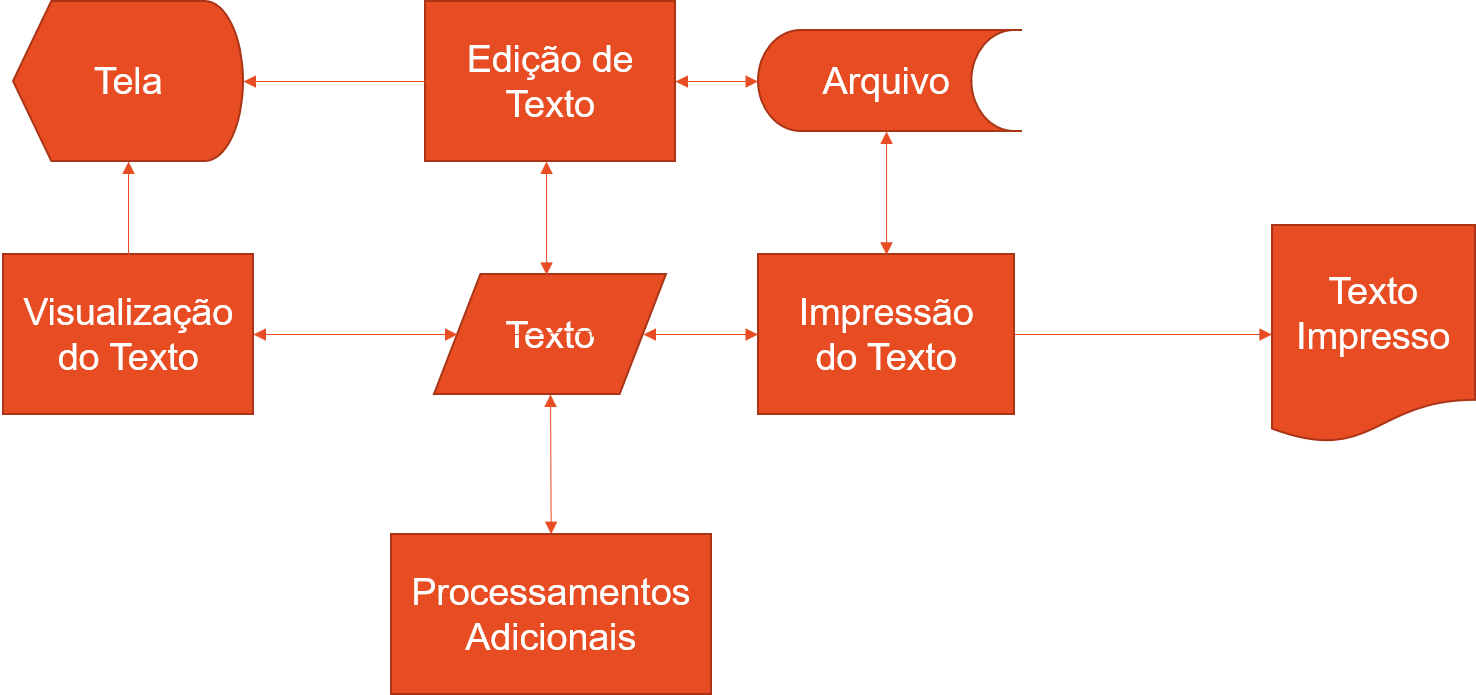
\includegraphics[width=0.7\linewidth]{Images/cadeia}
    \caption[A cadeia de processamento de texto]{A cadeia de processamento de texto}
    \label{fig:cadeia}
\end{figure}

\section{Tipos de Sistema de Processamento de Texto}

\subsection{Editores de Texto}

Editores de texto são programas que permitem ao usuário editar arquivos que são de \textbf{texto puro}. Texto puro é um conceito que mudou. Inicialmente significava que havia um mapeamento um para um entre o que você encontrava no arquivo, uma sequência de caracteres codificados em ASCII\footnote{ASCII é um padrão que associa uma letra, e outros símbolos usados em arquivos, a um byte. Seu nome significa American Standard Code for Information Interchange. Baseado no alfabeto inglês, originalmente usava apenas 128 símbolos (7 bits), não possuindo os caracteres acentuados de outras línguas.}. Em ASCII, por exemplo, a letra \enquote{A} é representada pelos bits \enquote{1000001} e a \enquote{a} por \enquote{1100001}. Atualmente são usadas codificações que permitem que um caracter ou símbolo seja representado por uma sequência mais longa de bits, por meio de \textit{escape codes}, por exemplo UTF-8\footnote{Unicode Transformation Format, que permite codificar 1.112.064 símbolos}, o que significa que os editores de texto, normalmente, não representam mais perfeitamente o arquivo em disco. Os sistemas de codificação atuais são normalmente extensões do ASCII, isto é, os 128 códigos de 1 byte do ASCII original ainda são válidos. A figura \ref{fig:funedtexto} mostra a função de um editor de texto na cadeia de processamento de texto.

\begin{figure}[hbt]
    \centering
    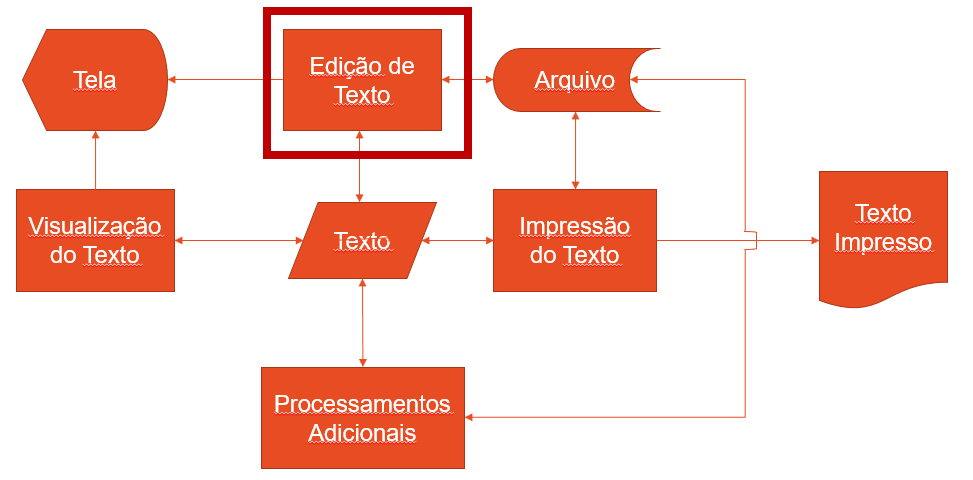
\includegraphics[width=0.7\linewidth]{Images/editordetexto}
    \caption[Função de um editor de texto]{Função de um editor de texto na cadeia de processamento de texto.}
    \label{fig:funedtexto}
\end{figure}





Editores de texto foram necessários assim que trocamos as entradas por cartão e fita, que eram editados em máquinas não conectadas ao computador, por terminais ligados diretamente aos mesmos. Os primeiros editavam linha a linha, a seguir outros exigiam que o usuário gerenciasse o \textit{buffer}, o seja, a parte do arquivo que estava em memória. Com o tempo chegamos a versões semelhantes as atuais.

Atualmente editores de texto tem um conjunto complexo de funções de busca, substituição, etc.

Exemplos de editores de texto atuais são o Notepad, que vem por \textit{default} com o Windows, o \texttt{vi} e o \texttt{vim}, Notepad++, EditPlus, TextEdit e o poderosíssimo Emacs. A figura \ref{fig:vim} mostra um exemplo to \texttt{vim}.


\begin{figure}[hbt]
    \centering
    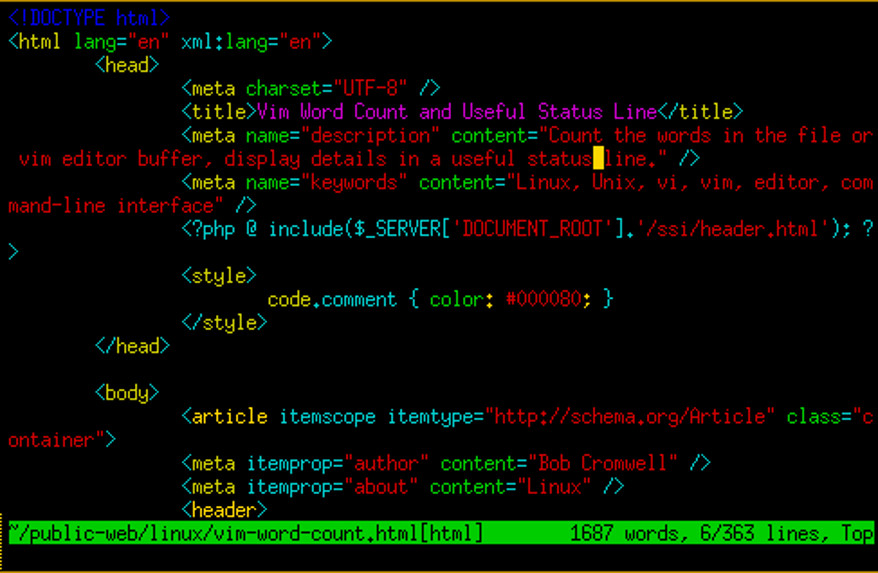
\includegraphics[width=0.7\linewidth]{Images/vim}
    \caption{O editor de texto vim}
    \label{fig:vim}
\end{figure}


\subsection{IDEs}

Uma IDE, ou \enquote{Integrated Development Environment}, é uma extensão lógica da ideia de editor de texto criada originalmente para programadores, fornecendo serviços adicionais a edição de texto, como compilação, \textit{debugging}, controle de versão, normalmente por meio de interfaces com os programas que fazem isso.

Uma IDE cobre a parte de edição e processamento de texto da cadeia de processamento de texto, como visto na figura \ref{fig:ide:cadeia}.

\begin{figure}[hbt]
    \centering
    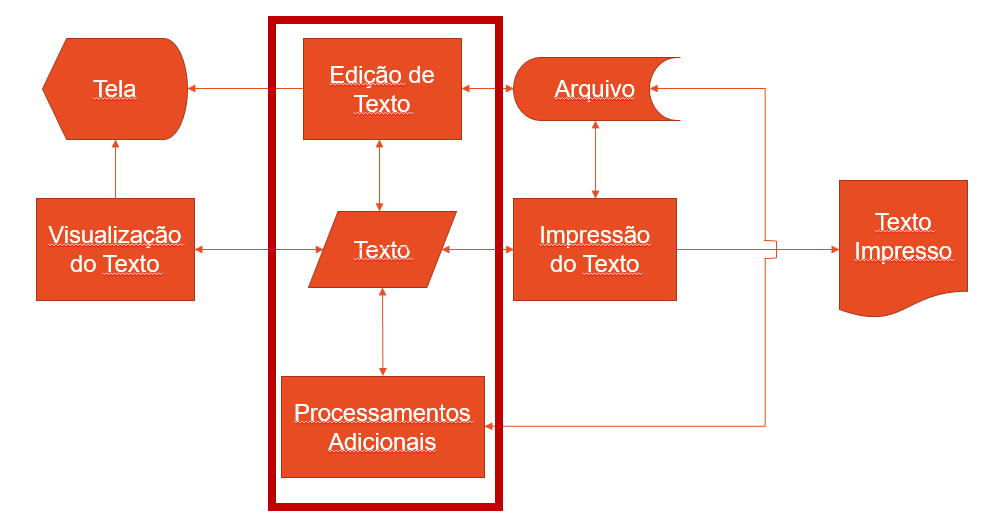
\includegraphics[width=0.7\linewidth]{Images/ide}
    \caption[Um IDE permite editar e invocar outros processsamentos de texto]{Um IDE permite editar e invocar outros processsamentos de texto}
    \label{fig:ide:cadeia}
\end{figure}



Exemplos de IDE são o Atom, o Visual Studio, o \TeX Studio e o próprio Emacs. Com a evolução dos editores de texto, a fronteira entre editores e IDEs ficou  indefinida, muitas vezes dependendo do uso que o usuário faz do programa. A figura \ref{fig:texstudio} mostra um exemplo do \TeX Studio.




\begin{figure}[hbt]
    \centering
    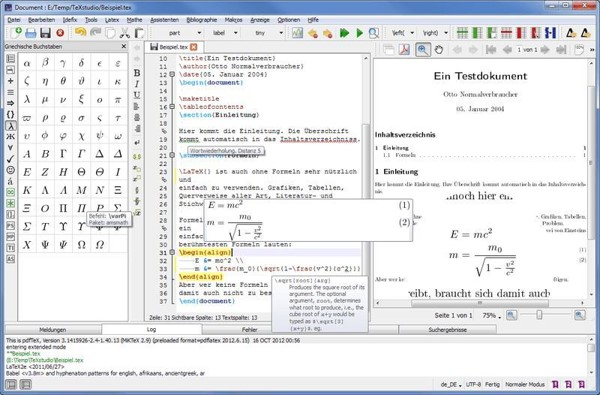
\includegraphics[width=0.7\linewidth]{Images/Picture1}
    \caption{O \TeX\ Studio}
    \label{fig:texstudio}
\end{figure}

\subsection{Sistemas de Tipografia}

Já que era possível editar textos, porque não imprimi-los de forma adequada? Essa ideia levou a criação de programas de tipografia, que faziam a tradução de um arquivo texto, com marcações adequadas, para um outro arquivo que fosse interpretado em uma impressora (ou outras máquinas mais sofisticadas de \textit{typesetting} dgital). 

Um sistema de tipografia cobre apenas a parte de impressão da cadeia de processamento de texto, como visto na figura \ref{fig:sisttipo1}.

\begin{figure}[hbt]
    \centering
    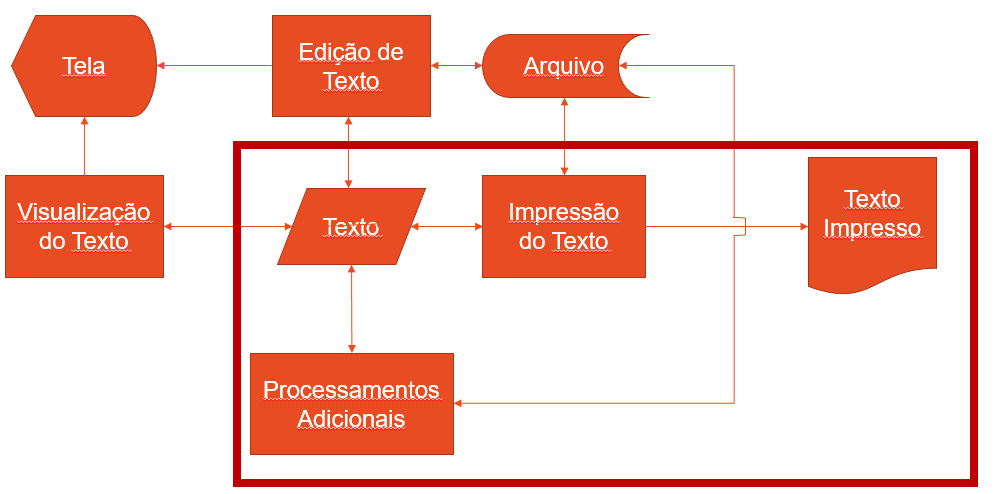
\includegraphics[width=0.7\linewidth]{Images/latex1}
    \caption[Sistemas de tipografia]{Sistemas de tipografia imprimem e fazem processamentos adicionais.}
    \label{fig:sisttipo1}
\end{figure}


Essas marcações adequadas são como comandos, e um arquivo de texto marcado se assemelha a um programa de computador, por possuir palavras código que dão os comandos necessários. Sistemas desse tipo não possuem editores associados e são normalmente ativados por linha de comando.

Exemplos de sistemas de tipografia são o troff, o \TeX\ e o \LaTeX. A figura \ref{fig:latex2} mostra o \LaTeX sendo usado em linha de comando.

\begin{figure}[hbt]
    \centering
    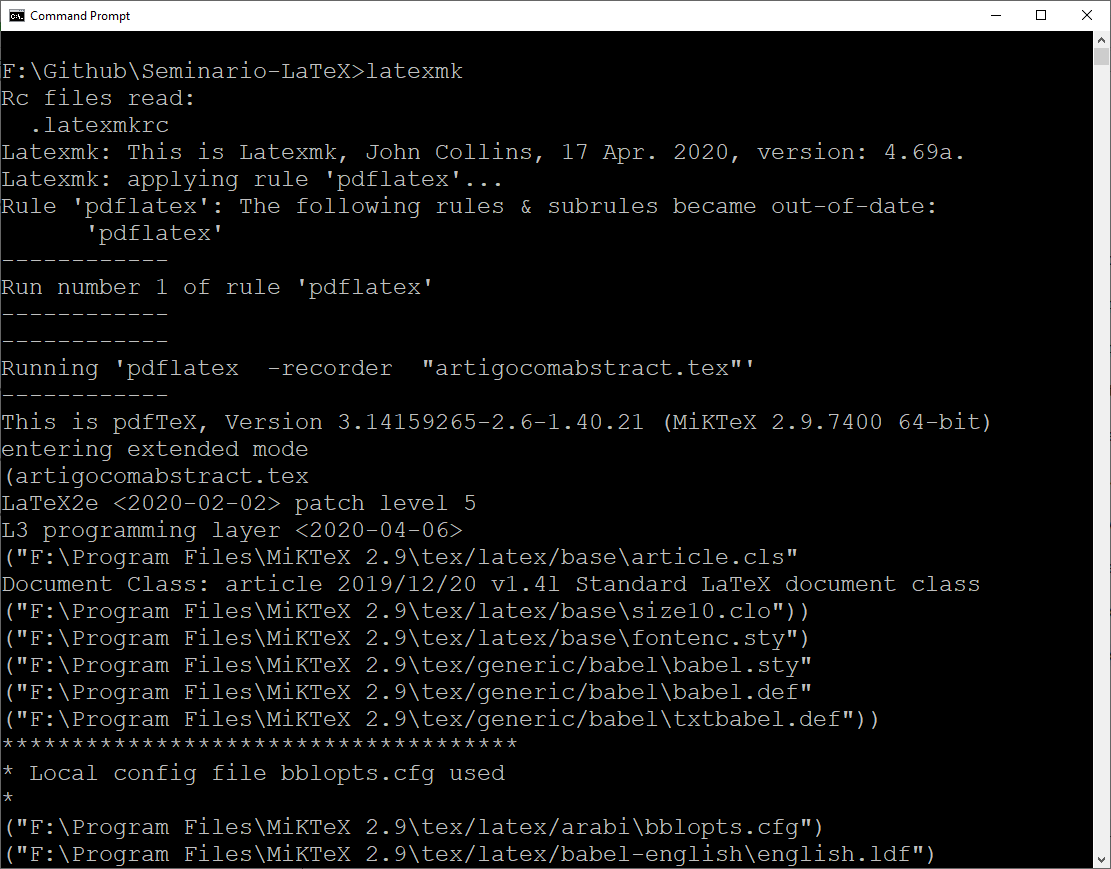
\includegraphics[width=0.7\linewidth]{Images/latex2}
    \caption[O \LaTeX sendo usado]{O \LaTeX sendo usado}
    \label{fig:latex2}
\end{figure}

\subsection{Processadores de Texto}

Principalmente com o advento do micro-computador, ficou claro que uma das principais utilidades do computador seria permitir a criação de textos a serem publicados, logo um editor de texto deveria ser estendido para suportar funções como colocar palavras em negrito, itálico, selecionar fontes, etc.

Processadores de texto cumprem grande parte das funções na cadeia de processamento de texto, como mostra a figura \ref{fig:processador}.

\begin{figure}[hbt]
    \centering
    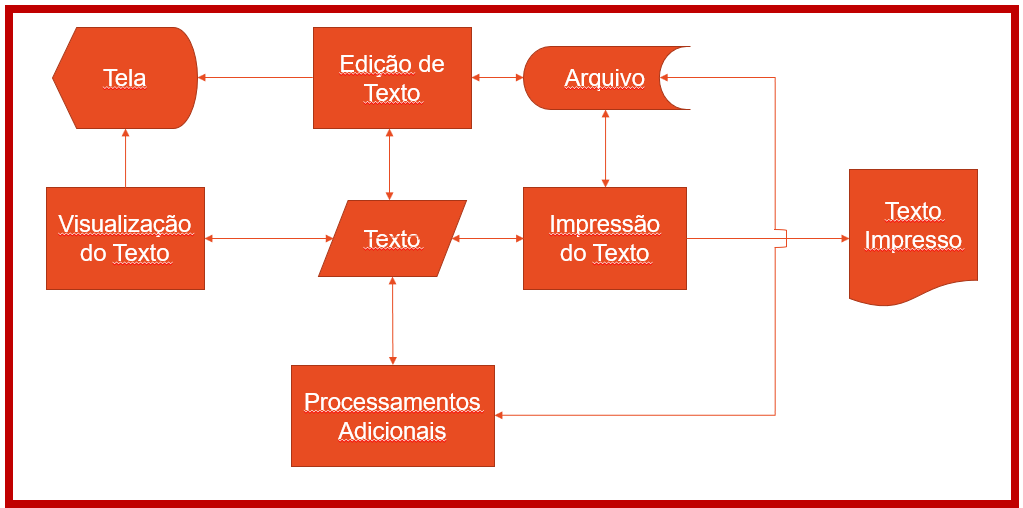
\includegraphics[width=0.7\linewidth]{Images/processador}
    \caption[Os processadores de texto]{Os processadores de texto na cadeia de processamento de texto.}
    \label{fig:processador}
\end{figure}

Com a evolução dos terminais de computadores, micro-computadores e placas de vídeo e monitores, os processadores de texto evoluíram de sistemas que mostravam alguma coisa do que estava sendo prevista para o texto, como caracteres em bold, para sistemas que permitiam uma visualização prévia, até chegar a edição pelo conceito de WYSIWYG, lido \enquote{uiziwig},  que mostra na tela quase que exatamente o que será visto na edição final, sendo as diferenças mínimas e quase imperceptíveis causadas por questões tecnológicas e da diferença entre papel e tintas e monitores.


Atualmente o Word é o processador de texto que domina amplamente o mercado, e seus principais concorrentes são sistemas de código aberto, como o LibreOffice Writer ou o Apache OpenOffice Writer. Um tela do Word é mostrada na figura \ref{fig:word}.

\begin{figure}[hbt]
    \centering
    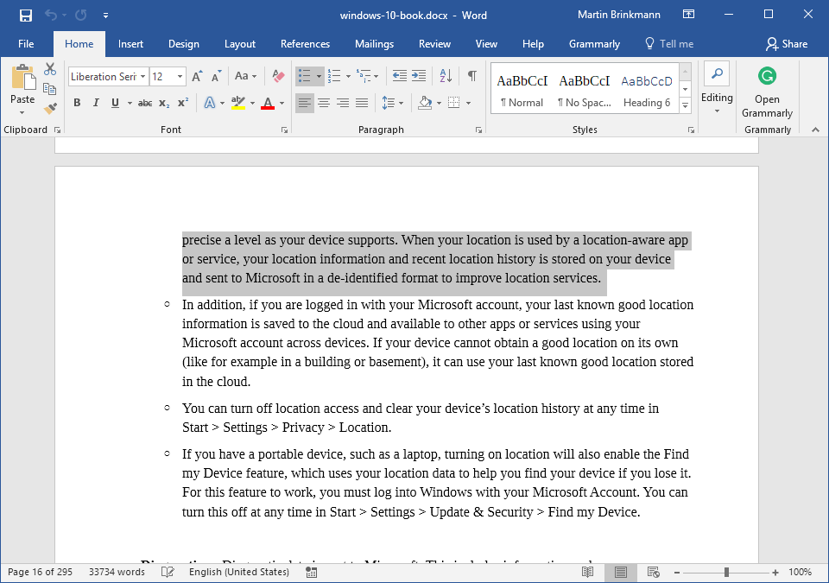
\includegraphics[width=0.7\linewidth]{Images/word}
    \caption[O Word]{O Word é o principal processador de texto do mercado.}
    \label{fig:word}
\end{figure}



\subsection{Sistemas de Autoria}

Sistemas de autoria são uma evolução interessante dos processadores de texto, ou dos IDEs, voltadas para autores de livros, roteiros, etc. que não só permitem editar o texto, em formatos específicos, como também guardar informações como fichas de personagens, descrições de cena, \textit{storyboards}, etc... Eles podem cobrir toda a cadeia de processamento de texto.

Exemplo de sistemas de autoria são o Scrivener, apresentado na figura \ref{fig:scrivener}, o Final Draft e o Celtx.

\begin{figure}[hbt]
    \centering
    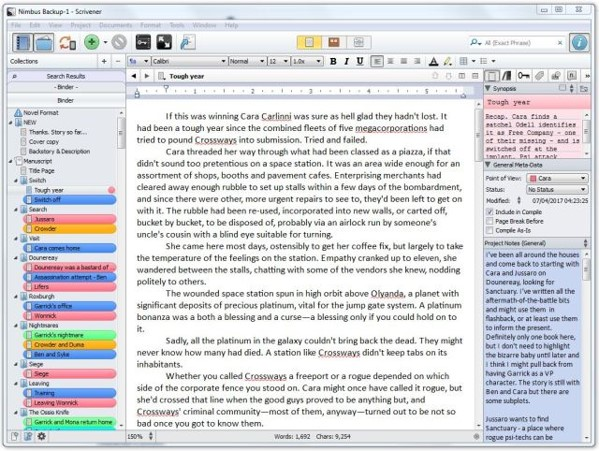
\includegraphics[width=0.7\linewidth]{Images/scrivener}
    \caption[Uma tela do Scrivener]{Uma tela do Scrivener}
    \label{fig:scrivener}
\end{figure}


\subsection{Sistemas Colaborativos de Edição}

Esses sistemas aparecem cedo, porém se expandem principalmente com o fortalecimento da internet. Eles permitem que mais de uma pessoa edite um arquivo ao mesmo tempo. Atualmente o mais conhecido é o Google Docs, que é um processador de texto limitado em funcionalidade mas muito fácil de usar.

O ShareLateX foi um sistema colaborativo de edição voltado para o \LaTeX\ que acabou sendo responsável por um renascimento do uso do \LaTeX\  na academia. Acabou sendo incorporado ao concorrent Overleaf, que aparece na figura \ref{fig:overleaf}.

\begin{figure}[hbt]
    \centering
    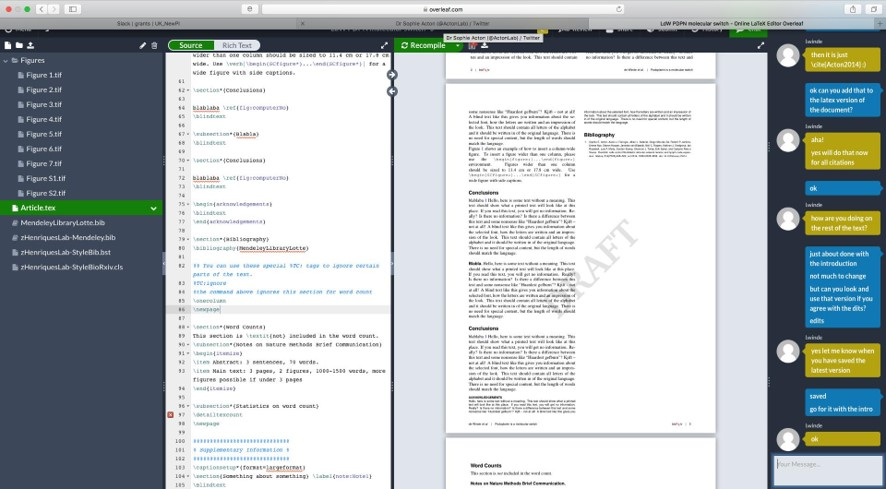
\includegraphics[width=0.7\linewidth]{Images/overleaf}
    \caption[O Overleaf]{O Overleaf.}
    \label{fig:overleaf}
\end{figure}

\subsection{O que é o \LaTeX}

\LaTeX é um sistema de typesetting baseado no \TeX e apoiado com outros programas, como o \hologo{biber} que permite usar arquivos de texto marcados para criar arquivos a serem impressos, ou no formato PDF,  seguindo regras de composição  (\textit{typesetting}) e usando fontes detalhadamente criadas para reproduzir a qualidade de fontes utilizada na composição manual, incluindo especialmente as ligaduras, que são caracteres especiais que representam dois ou mais caracteres de forma visualmente mais elegantes, como mostradas na figura \ref{fig:ligatureslatex}.

\begin{figure}[hbt]
    \centering
    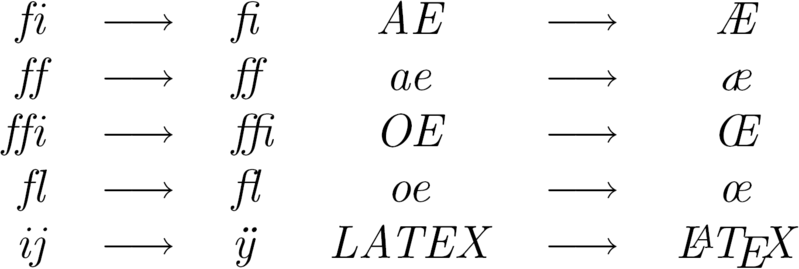
\includegraphics{Images/799px-LigaturesLatex}
    \caption[Exemplos de ligaturas de fontes do \TeX]{Exemplos de ligaturas de fontes do \TeX.}
    \label{fig:ligatureslatex}
\end{figure}









\end{document}